\chapter{Overview of the Cosmos SDK}
\label{OCS:overview}

In this chapter, we delve into the architecture of the Cosmos SDK, its modular components, and functionalities. We aim to shed light on both the advantages and the challenges faced by developers when employing this framework in blockchain development.

\section{High-level Overview}

The Cosmos SDK, an open-source framework, is instrumental in developing both permissioned \gls{poa} blockchains, like the Cosmos Hub\cite{cosmos-hub}, and multi-asset public \gls{pos} blockchains. The term "application-specific blockchain" is commonly used to describe blockchains crafted using the Cosmos SDK.

This approach diverges significantly from traditional virtual machine-based blockchains. Here, developers have full autonomy to make architectural decisions to optimize their application’s efficiency, performance, and security within a blockchain environment tailored for a single, specific use case. This flexibility is depicted in Listing~\ref{lst:app-based-blockchain}, highlighting the enhanced performance, security, and sovereignty achievable with application-specific blockchains.

\newpage
\begin{lstlisting}[language=bash, caption=Application based blockchains. Source:\cite{app-based-blockchain},label={lst:app-based-blockchain}]
                ^  +-------------------------------+  ^
                |  |                               |  |   Cosmos SDK
                |  |  State-machine = Application  |  |
                |  |                               |  v
                |  +-------------------------------+
                |  |                               |  ^
Blockchain node |  |           Consensus           |  |
                |  |                               |  |
                |  +-------------------------------+  |   CometBFT
                |  |                               |  |
                |  |           Networking          |  |
                |  |                               |  |
                v  +-------------------------------+  v
\end{lstlisting}

\section{Architecture}

Fundamentally, a blockchain functions as a replicated deterministic state machine. When provided with an initial state \(S\) and a transaction \(T\), it generates a new state \(S'\), as illustrated in Listing \ref{lst:state-transition}.

\begin{lstlisting}[language=bash, caption=State machine transition. Source:\cite{app-based-blockchain},label={lst:state-transition}]
                +--------+                 +--------+
                |        |                 |        |
                |   S    +---------------->+   S'   |
                |        |    apply(T)     |        |
                +--------+                 +--------+
\end{lstlisting}

To enhance processing efficiency, transactions are grouped into blocks. The state machine transitions from state \(S\) to \(S'\) by processing a block of transactions \(B\), as detailed in Listing \ref{lst:state-block-transition}.

\begin{lstlisting}[language=bash, caption=Block of bundled transactions. Source:\cite{app-based-blockchain},label={lst:state-block-transition}]
            +--------+                              +--------+
            |        |                              |        |
            |   S    +----------------------------> |   S'   |
            |        |   For each T in B: apply(T)  |        |
            +--------+                              +--------+
\end{lstlisting}

The Cosmos SDK empowers developers with extensive flexibility in defining their application's state, transaction types, and the processes for state transition. We will further explore how to construct state machines using the Cosmos SDK, starting with an analysis of how CometBFT facilitates state machine replication.

\subsection{CometBFT}

CometBFT serves as the agnostic engine for both the networking and consensus layers of a blockchain (as seen in Listing~\ref{lst:app-based-blockchain}). It is responsible for organizing and propagating transaction bytes. Relying on the \gls{bft} algorithm developed by Tendermint, CometBFT achieves consensus among network nodes.

Validators, unique nodes within the network, are pivotal to the CometBFT consensus process. They are responsible for updating the blockchain with new transaction blocks. At any given time, a set of validators \(V\) is active, with one validator selected as the proposer for the next block. A block is considered valid if over two-thirds of \(V\) have signed a prevote and a precommit for it, and if all included transactions are verified as genuine. The validator set can be altered based on rules defined within the state machine. The simplicity of this process is encapsulated in Figure \ref{fig:cometbft-overview}.

\begin{figure}[H]
    \centering
    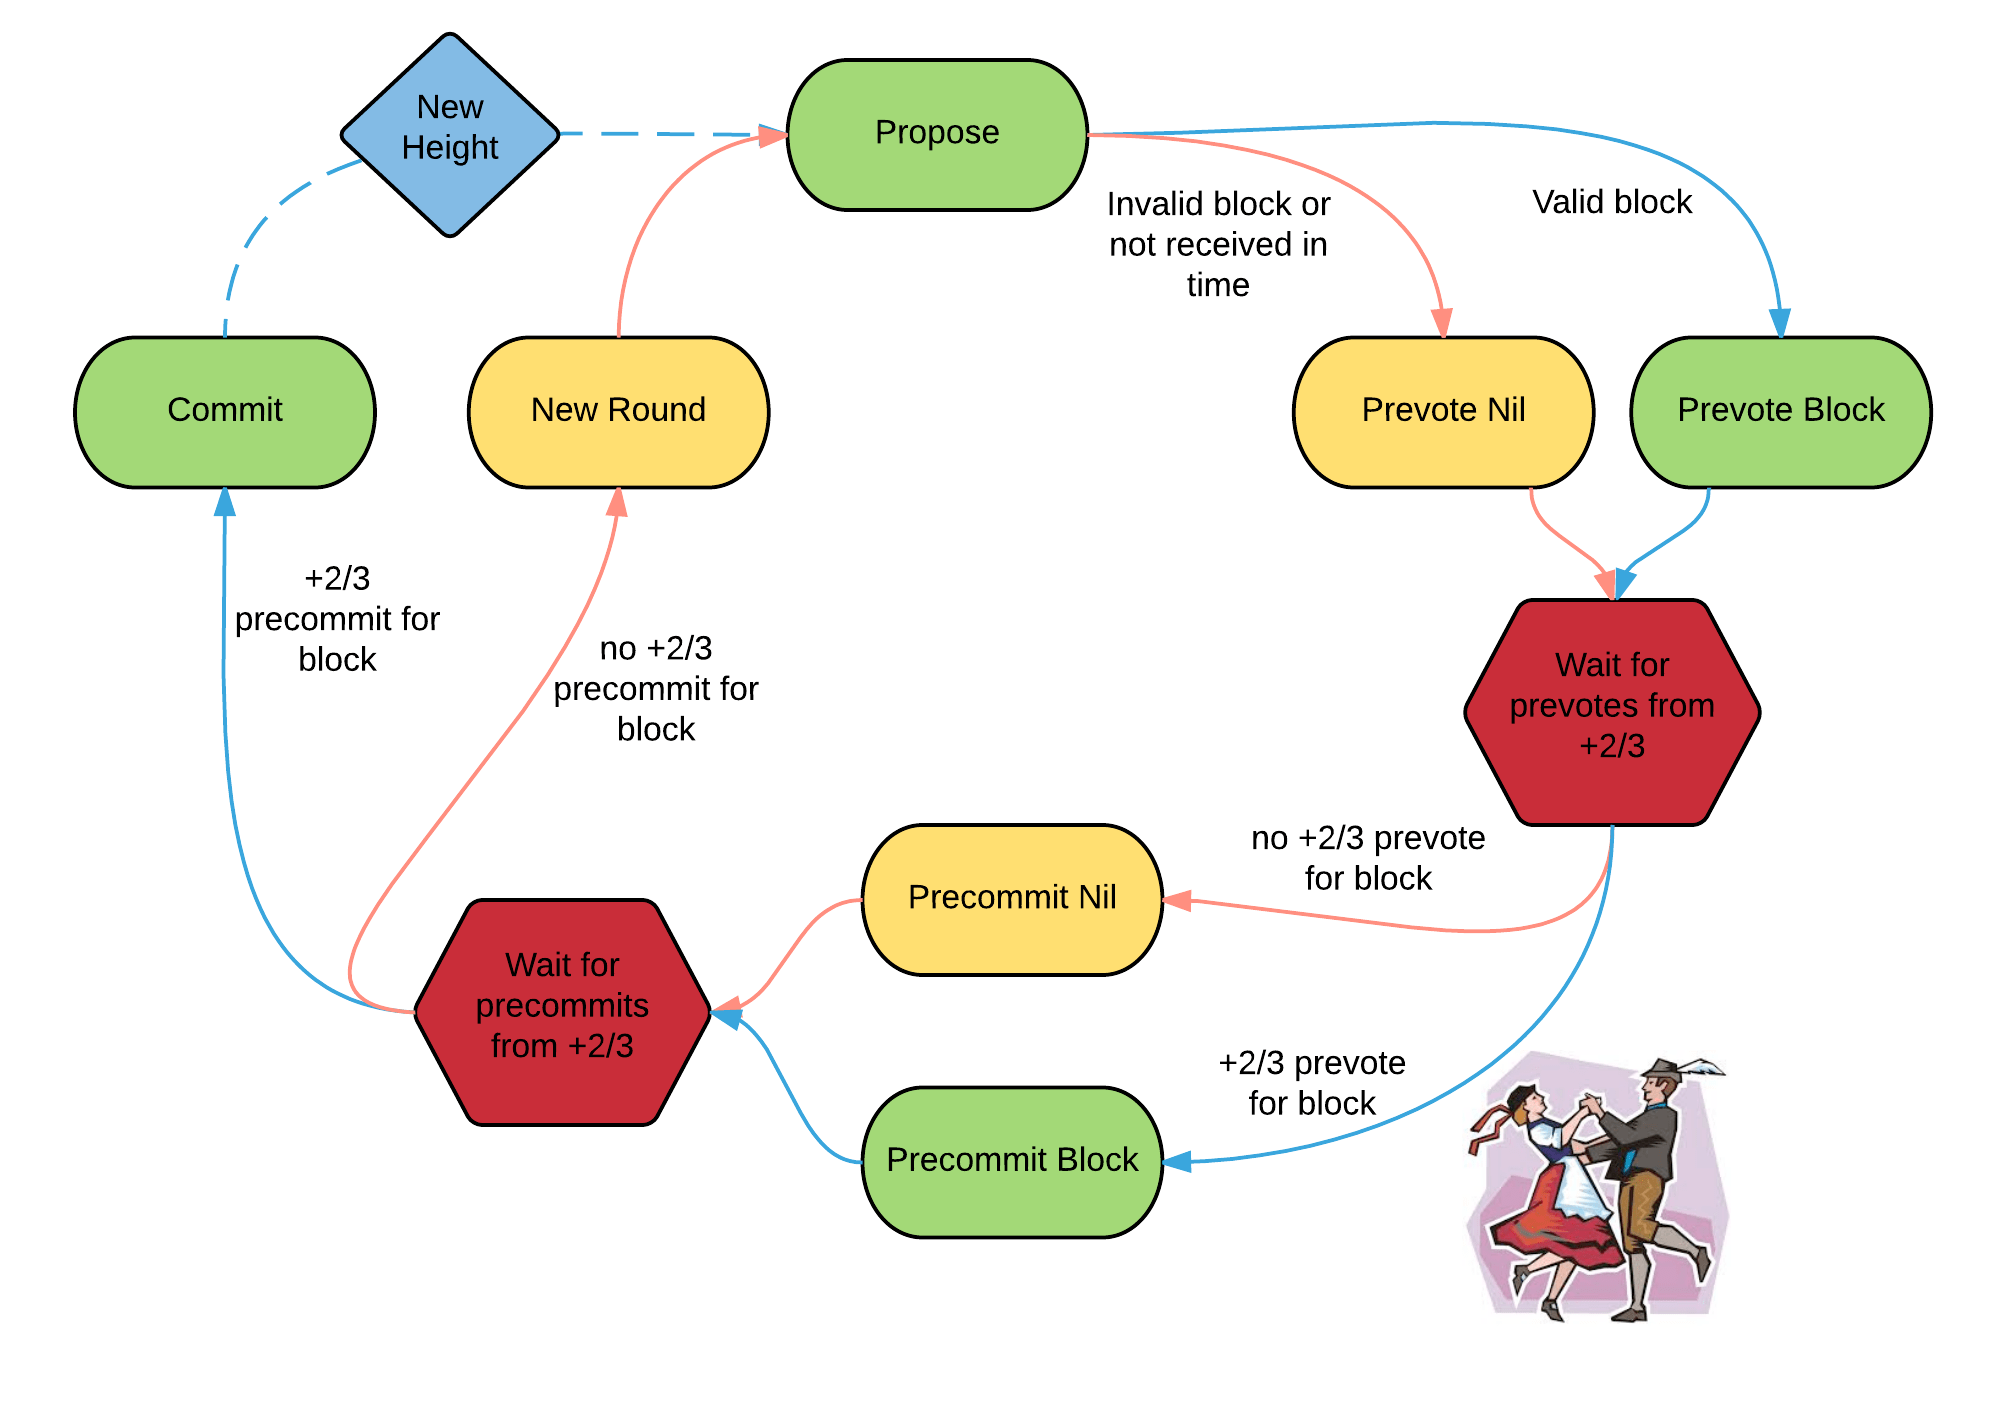
\includegraphics[width=\textwidth]{figures/cometbft.png}
    \caption{Consensus Overview CometBFT Source\cite{cometbft-overview}}
    \label{fig:cometbft-overview}
\end{figure}

\subsection{ABCI}

The \gls{abci} interface establishes standard protocols for communication between the consensus engine (CometBFT) and the application layer. This interface facilitates the separation of the consensus logic from application logic, significantly simplifying application development on the Cosmos SDK.

Through \gls{abci}, the consensus engine and the application interact seamlessly without needing to understand each other's internal mechanisms, as shown in Listing \ref{lst:ABCI}. This separation not only streamlines development but also promotes interoperability among various blockchain networks utilizing the Cosmos SDK.

\newpage
\begin{lstlisting}[language=bash, caption=ABCI Interface. Source:\cite{app-based-blockchain},label={lst:ABCI}]
                      +---------------------+
                      |                     |
                      |     Application     |
                      |                     |
                      +--------+---+--------+
                               ^   |
                               |   | ABCI
                               |   v
                      +--------+---+--------+
                      |                     |
                      |                     |
                      |       CometBFT      |
                      |                     |
                      |                     |
                      +---------------------+
\end{lstlisting}

\section{Applications Architecture}
\label{ch:applicatoins-architecture}

The Cosmos SDK's modular and decoupled architecture is a cornerstone of its design, enabling developers to focus primarily on application logic. The framework's 'baseApp' serves as a basic template, implementing necessary methods for routing transactions to different modules and facilitating communication with the CometBFT engine via \gls{abci} methods.

Modules in the Cosmos SDK act like smaller state machines within the larger blockchain state machine. They define both a segment of the state and specific message types. The 'BaseApp' routes these messages, and the modules interpret them using protobuf definitions, translating byte transactions managed by CometBFT into actionable application logic.

Fig \ref{fig:application-modules} illustrates the general architecture of the application layer. Here, the Cosmos SDK's core handles the essential connections and module composition, while custom modules developed using the SDK implement the primary functionalities of the application.

\begin{figure}[H]
    \centering
    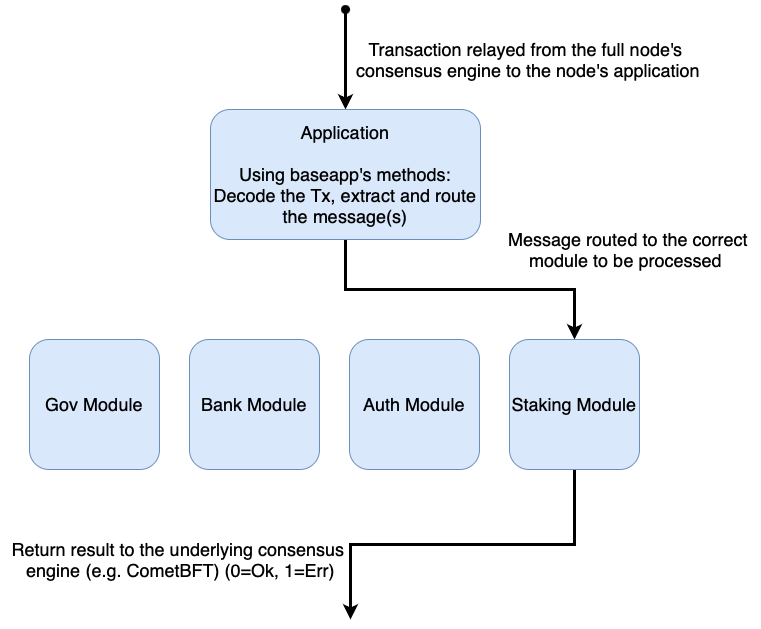
\includegraphics[width=\textwidth]{figures/prueba.png}
    \caption{Application architecture}
    \label{fig:application-modules}
\end{figure}
